\documentclass[a4paper]{article}

\usepackage[english]{babel}
\usepackage[utf8]{inputenc}
\usepackage{amsmath}
\usepackage{graphicx}
\usepackage[colorinlistoftodos]{todonotes}
\usepackage{amsmath,amsfonts,amssymb}
\usepackage{float}
\usepackage{tikz}
\usetikzlibrary{bayesnet}
\usetikzlibrary{fit, positioning, arrows.meta}
\usepackage[makeroom]{cancel}
\tikzset{
neuron/.style={shape=circle, minimum size=1.2cm,  inner sep=0, draw, font=\small}, io/.style={neuron, fill=gray!20}, deterministic/.style={diamond, minimum size=1.4cm, draw, text badly centered, inner sep=3pt}}

\title{Master Project: Notes}

\author{Tristan Guigue}

\date{\today}

\begin{document}
\maketitle

\section{Mutual Information and Maximum Likelihood in Supervised Setting}

We consider the simplest graphical model in a supervised learning setting:

\begin{center}
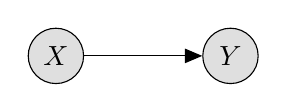
\begin{tikzpicture}
    \node[obs] (x) {$X$} ; 
    \node[obs, right=1.5cm of x] (y) {$Y$} ; 
    \draw [->] (x) -- (y) ; 
\end{tikzpicture}
\end{center}

We would like to check that maximising the mutual information between X and Y is equivalent to maximum likelihood:

\begin{align}
E_{X, Y}(\log p(y|x)) &= \int p(x, y)\,p(y| x)\, dx\,dy\\ 
&= - H(Y | X)\
\end{align}


\begin{align}
I(X, Y) &= H(Y) - H(Y|X)
\end{align}

So if we consider the entropy of the labels fixed, maximising the mutual information is indeed equivalent to maximum likelihood.

\section{Mutual Information Maximisation in Stochastic Feed-forward Network}

We consider a graphical model in a supervised learning setting:

\begin{figure}[H]
  \centering
  \tikz{ %
    \node[obs] (x) {$X$} ; %
    \node[latent, right=of x] (z) {$Z$} ; %
    \node[obs, right=of z] (y) {$Y$} ; %
    \edge {x} {z} ; %
    \edge {z} {y} ; %
  }
\end{figure}

Where X is our observed data and Y our labels. Z is a stochastic representation of our data.

\subsection{Maximum Likelihood}

We try to maximise the likelihood $\log p(y|x)$

\subsubsection{Naive approach}

The simplest way to do this would be to sample directly from the likelihood:

\begin{align}
 p(y|x) &= \int p(y, z|x) dz \\
 &= \int p(y|z) p(z|x) dz \\
 &= E_{Z | X}[p(y|z)] 
\end{align}

For example:
$$ p(y|z) = S(y | Wz + b) $$ were S is the softmax function.
And:
$$ p(z|x) \sim \mathcal{N}(z | f^\mu(x), f^\Sigma(x))$$ where $f^\mu$ and $f^\Sigma$ are multi-layer perceptrons.

We can approximate
\begin{align}
 p(y|x) &\approx \frac{1}{M} \sum^M_{m=1} p(y | z^{(m)}) 
\end{align}

Where $ z^{(m)} \sim p(z|x) $

However this might lead to a high variance because we can't be sure that our draw from $p(z | x)$ will contribute significantly to our estimate $p(y |x)$.

\subsubsection{Stochastic Gradient Variational Bayes}

To prevent this, we use a variational lower bound on the log likelihood:
\begin{align}
 \log p(y|x) &= \log(\int p(y, z|x) dz) \\
 & =  \log(\int q(z) \frac{p(y, z|x)}{q(z)}) \\
 & \geq \int q(z) \log \frac{p(y, z|x)}{q(z)}
\end{align}

Using Jensen's inequality.

\begin{align}
 \log p(y|x) & \geq \int q(z) \log \frac{p(z|x) p(y| z)}{q(z)} \\
  &= \int q(z) \log \frac{p(z|x)}{q(z)}  + \int q(z) \log p(y|z) \\
  &= E_q[p(y|z)] - KL[q(z) || p(z|x)]\\
  &\approx  \frac{1}{M} \sum^M_{m=1} p(y | z^{(m)}) - KL[q(z) || p(z|x)]
\end{align}
Where $ z^{(m)} \sim q(z)$ and assuming the KL divergence can be computed analytically.

So we try to maximise the expected value of decoder given z sampled from a distribution parametrised by the encoder while minimising the KL divergence between $q(z)$ and $p(z|x)$.

\subsection{Maximum Mutual Information}

We would like to compare this result to the maximisation of the  mutual information between Z and Y:

\begin{align}
I(Z, Y) &= \int p(y, z) \log \frac{p(z, y)}{p(z)p(y)} dy\,dz\\
& = \int p(y, z) \log \frac{p(y|z)}{p(y)} dy\,dz\\
&= \int p(y, z) \log p(y|z) dy\,dz - H(y) 
\end{align}
We ignore the entropy of the labels as it can't be maximised. We get:
\begin{align}
I(Z, Y) &= \int p(x, y, z) \log p(y| z) dx\,dy\,dz\\
&= \int p(z | x, y) p(x, y) \log p(y | z) dx\,dy\,dz
\end{align}
We can approximate the joint distribution of the data and the labels by:
$$ p(x, y) \approx \frac{1}{N}\sum_n \delta_{x_n}(x) \delta_{y_n}(y)$$
So we get:
$$ I(Z, Y) \approx \frac{1}{N} \int p(z | x^{(n)}, y^{(n}) \log p(y^{(n)} | z) $$

As we can see this is not equivalent to the maximum likelihood. In particular we have no way to easily get the posterior over z.

\section{Information Bottleneck in Recurrent Neural Networks}

For a stochastic feed-forward network we try to be maximally compressive on the input while being maximally informative on the output. In mutual information this translates to the objective funtion:

$$ J = I(Z, Y) - \beta I(X, Z)$$ under the graphical model

\begin{center}
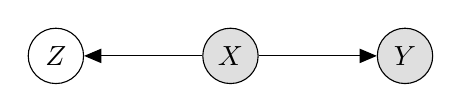
\begin{tikzpicture}
    \node[obs] (x) {$X$} ; 
    \node[obs, right=1.5cm of x] (y) {$Y$} ; 
    \node[latent, left=1.5cm of x] (z) {$Z$} ; 
    \draw [->] (x) -- (y) ; 
    \draw [->] (x) -- (z) ; 
\end{tikzpicture}
\end{center}

Applying this idea to a recurrent network we use the following graphical model:

\begin{figure}[H]
\centering
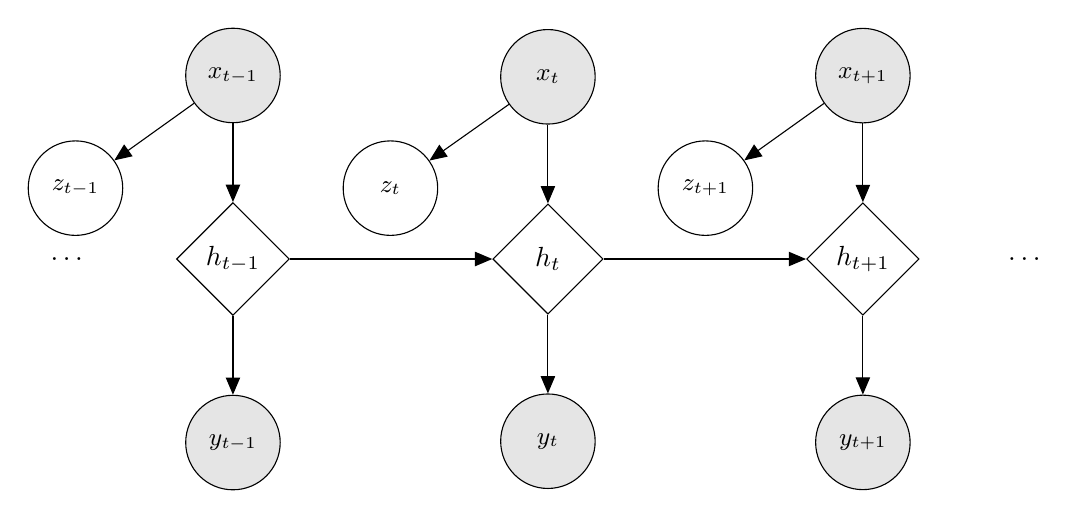
\begin{tikzpicture}[x=2cm, y=1.5cm]
\foreach \jlabel [count=\j, evaluate={\jj=int(\j-1); \jd=int(2 * \j);}]  in {t-1,  t, t+1}{
      \node [deterministic] at (\jd, 1) (h-\j) {$h_{\jlabel}$};
       \node [neuron] at (\jd - 1, 1.6) (z-\j) {$z_{\jlabel}$};
      \node [io, above=of h-\j] (x-\j) {$x_{\jlabel}$};
      \node [io, below=of h-\j] (y-\j) {$y_{\jlabel}$};
      \draw [->] (x-\j) -- (h-\j);
      \draw [->] (x-\j) -- (z-\j);
      \draw [->] (h-\j) -- (y-\j);
      \ifnum\j>1
          \draw [->] (h-\jj.east) -- (h-\j.west);
      \fi
} 
\node [left=of h-1] {\ldots};
\node [right=of h-3] {\ldots};
\end{tikzpicture}
\end{figure}

There are several mutual information objectives possible: 
For example we can take $$ J = \sum_t I(Z_t, Y_t) - \beta I(X_{1:t}, Z_t)$$ but we could also take
$$ J = \sum_t I(Z_t, Y_t) + I(Z_t, Y_{t+1:N}) - \beta I(X_{1:t}, Z_t)$$
 
Using the results from Alemi et al. \cite{vib} for the stochastic feed forward network, the objective function becomes: 
 
 $$ J = \frac{1}{TN} \sum_{t=1}^T \sum_{n=1}^{N} \mathbb{E}_{\epsilon \sim p(\epsilon)}[-\log q(y_{n,t} |f(x_{n,t}, \epsilon))] + \beta KL[p(Z|x_{n, t}), r(Z)]$$
 
 Note that we use the reparametrisation trick: $z = \mu + \sigma \epsilon$ where $\epsilon \sim \mathcal{N}(0, I)$ to be able to propagate the gradient through the encoder. 
 
 As previously we have:
$$ p(z_t|x_t) \sim \mathcal{N}(z_t | f^\mu(x_t), f^\Sigma(x_t))$$ where $f^\mu$ and $f^\Sigma$ are multi-layer perceptrons. The output of the perceptrons is divided in two, the first half gives the mean, we apply a softplus to the second half which gives the diagonal standard deviation terms.

\subsection{Results}

We compared the behavior of networks run with different values of beta for both feedforward and recurrent networks. 

\subsubsection{Feed Forward Network}

Using the same parameters as in the Deep Variational Information Bottleneck: bottleneck layer of dimension K = 256 and multilayer perceptron with two hidden layer of dimensions 1024.

\begin{center}
\begin{tabular}{ c | c c }
 $\beta$ & 0 & $10^{-3}$ \\ 
 error &  2.38 &  1.41 \\  
\end{tabular}
\end{center}

\subsubsection{Recurrent Network}

In the recurrent network setting we generated both continuous and binary data with a given pattern and some noise.

\paragraph{Experiment 1}
The first experiment we did was using the following parameters

\begin{center}
\begin{tabular}{ c | c  }
 Training samples & 500 \\ 
 Test samples &  500 \\
 Sequence length & 30 \\
 Hidden units & 128 \\
 Bottleneck size & 64 \\
 Cell & Single layer RNN
\end{tabular}
\end{center}

The results we got for the loss for the different values of $beta$ are:
\begin{center}
\begin{tabular}{ c | c c }
 $\beta$ & 0 & $10^{-3}$ \\ 
  \hline
 loss & 0.4494 &  0.4203 \\  
\end{tabular}
\end{center}

Which confirms that the information bottleneck is successfully regularising.

\paragraph{Experiment 2}
\begin{center}
\begin{tabular}{ c | c  }
 Training samples & 1000 \\ 
 Test samples &  1000 \\
 Sequence length & 60 \\
 Hidden units & 128 \\
 Bottleneck size & 64 \\
 Cell & Single layer RNN
\end{tabular}
\end{center}

\begin{center}
\begin{tabular}{ c | c c c c}
 $\beta$ & 0 & $10^{-3}$ & $10^{-2}$ & $10^{-1}$ \\ 
  \hline
 loss & 0.3696 &  0.3836  &  0.3691  &  0.3641 \\  
\end{tabular}
\end{center}

\paragraph{Experiment 3}
\begin{center}
\begin{tabular}{ c | c  }
 Training samples & 500 \\ 
 Test samples &  500 \\
 Sequence length & 60 \\
 Hidden units & 128 \\
 Bottleneck size & 64 \\
 Cell & Single layer LSTM
\end{tabular}
\end{center}

\begin{center}
\begin{tabular}{ c | c c }
 $\beta$ & 0 & $10^{-2}$ \\ 
  \hline
 loss & 0.3733 & 0.3628  \\  
\end{tabular}
\end{center}

\paragraph{Experiment 4}
\begin{center}
\begin{tabular}{ c | c  }
 Training samples & 500 \\ 
 Test samples &  500 \\
 Sequence length & 60 \\
 Hidden units & 128 \\
 Bottleneck size & 32 \\
 Cell & Single layer GRU
\end{tabular}
\end{center}


\begin{center}
\begin{tabular}{ c | c c c c }
 $\beta$ & 0 & $10^{-3}$ & $5*10^{-3}$ & $10^{-2}$ \\ 
  \hline
 loss & 0.3613 & 0.3585 & 0.3580 & 0.3586  \\  
\end{tabular}
\end{center}

\paragraph{Experiment 6: MNIST}

We were not successful in applying the information bottleneck with MNIST: networks not regularised systematically outperformed regularised ones.

\begin{center}
\begin{tabular}{ c | c  }
Data & MNIST \\
 Training samples & 500 \\ 
 Test samples &  500 \\
 Sequence length & 60 \\
 Hidden units & 128 \\
 Bottleneck size & 32 \\
 Cell & Single layer GRU
\end{tabular}
\end{center}


\begin{center}
\begin{tabular}{ c | c c c c c c}
 $\beta$ & 0 & $10^{-4}$ & $5*10^{-3}$ & $10^{-2}$ & $10^{-1}$ & 1 \\ 
 \hline
 loss & 0.1812 & 0.1829 & 0.187 & 0.1917 & 0.2005 & 0.2094 \\  
\end{tabular}
\end{center}

We tried to vary the parameters one by one with different values of beta with no success:
\begin{center}
\begin{tabular}{ c | c c }
$\beta$  & 0 & $5*10^{-3}$  \\
\hline
Sequence length: 100 & 0.1539 & 0.1577 \\
Sequence length: 200 & 0.1459 & 0.1505 \\
Sequence length: 784 & 0.08737 & 0.08749 \\
Train samples: 200 & 0.1908 & 0.1956 \\
Train samples: 1000 & 0.1803 & 0.1837 \\
Bottleneck: 64 & 0.1850 & 0.1913 \\
Bottleneck: 16 & 0.185 & 0.191 \\
Cell: RNN & 0.1832 & 0.19 \\
Hidden layer: 256 & 0.1851 & 0.1901 \\
Data: Single label 1 & 0.06650 & 0.06905 \\
\end{tabular}
\end{center}




\subsection{Differentiable prior}

To improve the expressiveness of the prior distribution on the latent, we allow its parameters to be learned. 

$$p(z) \sim \mathcal{N}(\mu_p, \Sigma_p)$$

The KL divergence between 2 gaussians with diagonal variance:

\begin{align}
KL(\mathcal{N}_q, \mathcal{N}_p) &= \frac{1}{2}(Tr(\Sigma_p^{-1}\Sigma_q) + (\mu_p - \mu_q)^T\Sigma_p^{-1}(\mu_p - \mu_q) - k + \log\frac{|\Sigma_p|}{|\Sigma_q|})\\
&= \frac{1}{2}(\sum_i \frac{\Sigma_{q, ii}}{\Sigma_{p, ii}} + \sum_i \frac{(\mu_{p_i} - \mu_{q, i})^2}{\Sigma_{p, ii}} - k + \log\frac{\prod \Sigma_{p, ii}}{\prod \Sigma_{q, ii}})\\
&= \frac{1}{2}(\sum_i[ \log \Sigma_{p, ii} - \log \Sigma_{q, ii} - 1 + \frac{\Sigma_{q, ii}}{\Sigma_{p, ii}} + \frac{(\mu_{p_i} - \mu_{q, i})^2}{\Sigma_{p, ii}}]
\end{align}

Beforehand we had assumed a standard normal prior which gave:
\begin{align}
KL(\mathcal{N}_q, \mathcal{N}_0) &= \sum_i[ -\log \Sigma_{q, ii} - 1 + \Sigma_{q, ii}+ \mu_{q, i}^2]
\end{align}

With this improved prior we get a better test accuracy:

\begin{center}
\begin{tabular}{ c | c c }
 $\beta$ & 0 & $10^{-3}$ \\ 
 error &  2.38 &  1.32 \\  
\end{tabular}
\end{center}

\subsection{Sequence to sequence}

We now try to compress a partial sequence and retrieve a future sequence based on the compressed state.

The graphical model is then

\begin{center}
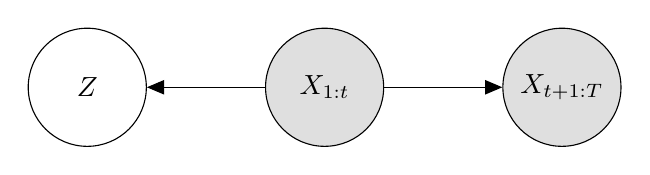
\begin{tikzpicture}
    \node[obs, minimum size=1.5cm] (x) {$X_{1:t}$} ; 
    \node[obs, right=1.5cm of x, minimum size=1.5cm] (y) {$X_{t+1:T}$} ; 
    \node[latent, left=1.5cm of x, minimum size=1.5cm] (z) {$Z$} ; 
    \draw [->] (x) -- (y) ; 
    \draw [->] (x) -- (z) ; 
\end{tikzpicture}
\end{center}

And the objective function


\section{Normalising Flow and Gradient Estimator without score function}

The variational lower bound can be writen as:

$$ \mathcal{L} = \mathbb{E}_{z \sim q}[\log p(x, z) - \log q_\phi(z|x)] $$

Taking a single Monte Carlo sample this becomes:

$$ \mathcal{L}_{mc} = \log p(x, z) - \log q_\phi(z|x) $$

The gradient with respect to the variational parameter is then:

\begin{align}
\Delta_{TD}(\epsilon, \phi) = \Delta_z[\log p(z|x) -  \log q_\phi(z|x)] \Delta_\phi t(\epsilon, \phi) - \Delta \log q_\phi(z|x)
\end{align}

Removing the score function we get another unbiased estimator that has lower variance when q is closed to the posterior:
$$ \Delta_{PD}(\epsilon, \phi) =  \Delta_z[\log p(z|x) -  \log q_\phi(z|x)] \Delta_\phi t(\epsilon, \phi)$$

A normalising flow is a powerful representation of the posterior though a succession of invertible transformation.

$$ z_K = f_K \circ ... \circ f_1(z_0)$$

And their normalised distribution:

$$ q_K(z_K) = q_0(z_0) \prod_{k=1}^K \lvert \frac{\partial f_k}{\partial z_{k-1}} \rvert^{-1}$$
$$\log  q_K(z_K) = \log q_0(z_0) -  \sum_{k=1}^K \log \lvert \frac{\partial f_k}{\partial z_{k-1}} \rvert$$

With
$$ q_0(z_0) \sim \mathcal{N}(q_0 | f^\mu(x), f^\Sigma(x))$$

The free energy lower bound is now:

\begin{align}
\mathcal{L} &= \mathbb{E}_{z \sim q}[\log p(x, z) - \log q_\phi(z|x)] \\
&=  \mathbb{E}_{z \sim q_0}[\log p(x, z_K) - \log q_K(z_K)] 
\end{align}

Sampling from $q_0$ we get:
$$ \mathcal{L}_{mc} = \log p(x, z_K) - \log q_K(z_K) $$

And the gradient:

\begin{align}
\Delta_\phi \mathcal{L}_{mc} &= \frac{\partial}{\partial \phi} \log p(x, z_K) - \frac{\partial}{\partial \phi}  \log q_K(z_K) \\
&= \Delta_{z_K}[\log p(x, z_K) - \log q_K(z_K)] \Delta_\phi z_K - \cancel{\Delta_\phi \log q_K(z_K)}
\end{align}

We'd like to use a neural network with leaky ReLu activation for $f$ since they have constant gradient. However the change of variable 
$$q(z^\prime) = q(f^{-1}(z^\prime)) \lvert \frac{\partial f}{\partial z} \rvert^{-1} $$ is only valid if $f$ is differentiable which is not the case here.




 \begin{thebibliography}{9}
\bibitem{vib} 
Alexander A. Alemi, Ian Fischer, Joshua V. Dillon, Kevin Murphy. 
\textit{Deep Variational Information Bottleneck}. 
ICLR, 2017.
\end{thebibliography}

 
\end{document}



